%%% The main file. It contains definitions of basic parameters and includes all other parts.

%% Settings for single-side (simplex) printing
% Margins: left 40mm, right 25mm, top and bottom 25mm
% (but beware, LaTeX adds 1in implicitly)
\documentclass[12pt,a4paper]{report}
\setlength\textwidth{145mm}
\setlength\textheight{247mm}
\setlength\oddsidemargin{15mm}
\setlength\evensidemargin{15mm}
\setlength\topmargin{0mm}
\setlength\headsep{0mm}
\setlength\headheight{0mm}
% \openright makes the following text appear on a right-hand page
\let\openright=\clearpage

%% Settings for two-sided (duplex) printing
% \documentclass[12pt,a4paper,twoside,openright]{report}
% \setlength\textwidth{145mm}
% \setlength\textheight{247mm}
% \setlength\oddsidemargin{14.2mm}
% \setlength\evensidemargin{0mm}
% \setlength\topmargin{0mm}
% \setlength\headsep{0mm}
% \setlength\headheight{0mm}
% \let\openright=\cleardoublepage

%% Generate PDF/A-2u
% disabled because I do not have a color profile
\usepackage[a-2u]{pdfx}

%% Character encoding: usually latin2, cp1250 or utf8:
\usepackage[utf8]{inputenc}

%% Prefer Latin Modern fonts
\usepackage{lmodern}

%% Further useful packages (included in most LaTeX distributions)
\usepackage{amsmath}        % extensions for typesetting of math
\usepackage{amsfonts}       % math fonts
\usepackage{amsthm}         % theorems, definitions, etc.
\usepackage{bbding}         % various symbols (squares, asterisks, scissors, ...)
\usepackage{bm}             % boldface symbols (\bm)
\usepackage{graphicx}       % embedding of pictures
\usepackage{fancyvrb}       % improved verbatim environment
\usepackage{natbib}         % citation style AUTHOR (YEAR), or AUTHOR [NUMBER]
\usepackage[nottoc]{tocbibind} % makes sure that bibliography and the lists
			    % of figures/tables are included in the table
			    % of contents
\usepackage{dcolumn}        % improved alignment of table columns
\usepackage{booktabs}       % improved horizontal lines in tables
\usepackage{paralist}       % improved enumerate and itemize
\usepackage[usenames]{xcolor}  % typesetting in color
\usepackage{gensymb} % the degree symbol

%%% Basic information on the thesis

% Thesis title in English (exactly as in the formal assignment)
\def\ThesisTitle{Software-based eye tracking}

% Author of the thesis
\def\ThesisAuthor{Adam Dominec}

% Year when the thesis is submitted
\def\YearSubmitted{2017}

% Name of the department or institute, where the work was officially assigned
% (according to the Organizational Structure of MFF UK in English,
% or a full name of a department outside MFF)
\def\Department{Department of Software and Computer Science Education}

% Is it a department (katedra), or an institute (ústav)?
\def\DeptType{Department}

% Thesis supervisor: name, surname and titles
\def\Supervisor{RNDr. Barbara Zitová, Ph.D.}

% Supervisor's department (again according to Organizational structure of MFF)
\def\SupervisorsDepartment{Institute of Information Theory and Automation, Czech Academy of Science}

% Study programme and specialization
\def\StudyProgramme{Computer Science}
\def\StudyBranch{Software Systems}

% An optional dedication: you can thank whomever you wish (your supervisor,
% consultant, a person who lent the software, etc.)
\def\Dedication{%
I am thankful to all the people who provided their face to my testing datasets, including those who do not know about it.
}

% Abstract (recommended length around 80-200 words; this is not a copy of your thesis assignment!)
\def\Abstract{%
This thesis presents a software library for eye gaze tracking.
The typical use case is a person watching their computer screen.
All data is obtained from a single video camera and is processed in real time.
The resulting software is freely available including source code.
}

% 3 to 5 keywords (recommended), each enclosed in curly braces
\def\Keywords{%
{face tracking} {gaze tracking} {image analysis}
}

%% The hyperref package for clickable links in PDF and also for storing
%% metadata to PDF (including the table of contents).
\hypersetup{unicode}
\hypersetup{breaklinks=true}
%\hypersetup{pdftitle={\ThesisTitle}}
%\hypersetup{pdfauthor={\ThesisAuthor}}
%\hypersetup{pdfkeywords=\Keywords}
\hypersetup{colorlinks=false, pdfborder={0 0 0}}

% Definitions of macros (see description inside)
%%% This file contains definitions of various useful macros and environments %%%
%%% Please add more macros here instead of cluttering other files with them. %%%

%%% Minor tweaks of style

% These macros employ a little dirty trick to convince LaTeX to typeset
% chapter headings sanely, without lots of empty space above them.
% Feel free to ignore.
\makeatletter
\def\@makechapterhead#1{
  {\parindent \z@ \raggedright \normalfont
   \Huge\bfseries \thechapter. #1
   \par\nobreak
   \vskip 20\p@
}}
\def\@makeschapterhead#1{
  {\parindent \z@ \raggedright \normalfont
   \Huge\bfseries #1
   \par\nobreak
   \vskip 20\p@
}}
\makeatother

% This macro defines a chapter, which is not numbered, but is included
% in the table of contents.
\def\chapwithtoc#1{
\chapter*{#1}
\addcontentsline{toc}{chapter}{#1}
}

% Draw black "slugs" whenever a line overflows, so that we can spot it easily.
\overfullrule=1mm

%%% Macros for definitions, theorems, claims, examples, ... (requires amsthm package)

\theoremstyle{plain}
\newtheorem{thm}{Theorem}
\newtheorem{lemma}[thm]{Lemma}
\newtheorem{claim}[thm]{Claim}
\newtheorem{definition}[thm]{Definition}

\theoremstyle{plain}
\newtheorem{defn}{Definition}

\theoremstyle{remark}
\newtheorem*{cor}{Corollary}
\newtheorem*{rem}{Remark}
\newtheorem*{example}{Example}

%%% An environment for proofs

%%% FIXME %%% \newenvironment{proof}{
%%% FIXME %%%   \par\medskip\noindent
%%% FIXME %%%   \textit{Proof}.
%%% FIXME %%% }{
%%% FIXME %%% \newline
%%% FIXME %%% \rightline{$\square$}  % or \SquareCastShadowBottomRight from bbding package
%%% FIXME %%% }

%%% An environment for typesetting of program code and input/output
%%% of programs. (Requires the fancyvrb package -- fancy verbatim.)

\DefineVerbatimEnvironment{code}{Verbatim}{fontsize=\small, frame=single}

%%% The field of all real and natural numbers
\newcommand{\R}{\mathbb{R}}
\newcommand{\N}{\mathbb{N}}
\renewcommand{\C}{\mathbb{C}}

%%% Useful operators
\DeclareMathOperator{\pr}{\textsf{P}}
\DeclareMathOperator{\E}{\textsf{E}\,}
\DeclareMathOperator{\var}{\textrm{var}}
\DeclareMathOperator{\cov}{\textrm{cov}}
\DeclareMathOperator{\sd}{\textrm{sd}}
\renewcommand{\vec}[0]{\textrm{vec}}
\newcommand{\diag}[0]{\textrm{diag}}

%%% Transposition of a vector/matrix
\def\T{^{\!\mathsf{T}}}
\def\inv{^{-\mathsf{I}}}

% Fraction written using a slash
\newcommand\smallfrac[2]{{}^{#1}\!/_{#2}}

%%% Various math goodies
\newcommand{\goto}{\rightarrow}
\newcommand{\gotop}{\stackrel{P}{\longrightarrow}}
\newcommand{\maon}[1]{o(n^{#1})}
\newcommand{\abs}[1]{\left|{#1}\right|}
\newcommand{\dint}{\int_0^\tau\!\!\int_0^\tau}
\newcommand{\isqr}[1]{\frac{1}{\sqrt{#1}}}

%%% Various table goodies
\newcommand{\pulrad}[1]{\raisebox{1.5ex}[0pt]{#1}}
\newcommand{\mc}[1]{\multicolumn{1}{c}{#1}}

%%% Matrix and vector
\renewcommand\vec[1]{\mathbf{#1}}
\newcommand{\mat}[1]{\mathtt{#1}}
\newcommand\hatvec[1]{\hat{\vec{#1}}}
\newcommand\hatmat[1]{\hat{\mat{#1}}}

% TODO pred odevzdanim prace je nutne zkontrolovat, ze toto makro se uz v textu nevyskytuje
\newcommand\todo[1]{(\textit{\underline{TODO:} #1})}


% Title page and various mandatory informational pages
\begin{document}
%%% Title page of the thesis and other mandatory pages

%%% Title page of the thesis

\pagestyle{empty}
\hypersetup{pageanchor=false}
\begin{center}

\centerline{\mbox{
\includegraphics[width=166mm]{img/logo-en.pdf}}}

\vspace{-8mm}
\vfill

{\bf\Large MASTER THESIS}

\vfill

{\LARGE\ThesisAuthor}

\vspace{15mm}

{\LARGE\bfseries\ThesisTitle}

\vfill

\Department

\vfill

\begin{tabular}{rl}

Supervisor of the master thesis: & \Supervisor \\
\noalign{\vspace{2mm}}
Study programme: & \StudyProgramme \\
\noalign{\vspace{2mm}}
Study branch: & \StudyBranch \\
\end{tabular}

\vfill

% Zde doplňte rok
Prague \YearSubmitted

\end{center}

\newpage

%%% Here should be a bound sheet included -- a signed copy of the "master
%%% thesis assignment". This assignment is NOT a part of the electronic
%%% version of the thesis. DO NOT SCAN.

%%% A page with a solemn declaration to the master thesis

\openright
\hypersetup{pageanchor=true}
\pagestyle{plain}
\pagenumbering{roman}
\vglue 0pt plus 1fill

\noindent
I declare that I carried out this master thesis independently, and only with the cited
sources, literature and other professional sources.

\medskip\noindent
I understand that my work relates to the rights and obligations under the Act No.~121/2000 Sb.,
the Copyright Act, as amended, in particular the fact that the Charles
University has the right to conclude a license agreement on the use of this
work as a school work pursuant to Section 60 subsection 1 of the Copyright Act.

\vspace{10mm}

\hbox{\hbox to 0.5\hsize{%
In ........ date ............	% FIXME!
\hss}\hbox to 0.5\hsize{%
signature of the author
\hss}}

\vspace{20mm}
\newpage

%%% Mandatory information page of the thesis

\openright

\vbox to 0.5\vsize{
\setlength\parindent{0mm}
\setlength\parskip{5mm}

Title:
\ThesisTitle

Author:
\ThesisAuthor

\DeptType:
\Department

Supervisor:
\Supervisor, \SupervisorsDepartment

Abstract:
\Abstract

Keywords:
\Keywords

\vss}

\newpage

%%% Dedication

\openright

\noindent
\Dedication

\newpage

\openright
\pagestyle{plain}
\pagenumbering{arabic}
\setcounter{page}{1}


%%% A page with automatically generated table of contents of the master thesis

\tableofcontents

%%% Each chapter is kept in a separate file
\chapter{Introduction}

The main idea behind this program is to view human eye as a means of communication.
It is rather intuitive for us to recognize other people's gaze just by looking at their face thanks to high contrast coloring of the eye itself.
The relevant brain circuitry develops early in infants and is equivalent among individuals.
This seems to be an evidence of evolutionary purpose---the human eye is built in a way so as to display the gaze clearly.
Therefore it should also be possible for a computer to estimate gaze from the data us humans have available, that is, a color image.

Thanks to the fact that almost every laptop computer or cell phone is now equipped with a video camera, the hardware requirements of this software are easy to satisfy.
Future programs built on top of this library will also exhibit minimal hardware requirements that enable them to be used almost immediately upon download and completely for free.

The possible applications are a vast topic.
Along the communication concept, eye trackers can be used for human-computer interaction.
Wide variety of algorithms have been proposed for on-screen keyboard and general desktop control \cite{majaranta02}.
In contrast to classical input devices, they make computers accessible to disabled users that have difficulty to move their limbs.
They can also improve the user comfort, such as by speeding up mouse motion in accordance to the gaze.

Running a gaze tracker quietly in the background (perhaps in a low quality) can also be helpful.
When the screen of a cell phone is not looked at, it can automatically lock to improve security.
On the other hand, it can display a message when somebody reads over your shoulder.

The gaze provides valuable information even when we do not concentrate on it.
In psychological experiments, it is often used as a synonym of the subject's attention.
An industrial application of this method is found in marketing and user experience design, where gaze recordings can be used to evaluate the quality of presentation of a product, or of an interface layout.
Knowing the user's center of attention can also serve as a cue for adaptive rendering in video games because the rest of the screen need not be displayed in full detail.
Tracking the gaze of a car driver can be used to improve safety \cite{murphy-chutorian07}.

\section{History}

Perhaps a more appropriate heading of this section would be \textit{Unrelated Work}.
Indeed, before we get to the overview of our software competitors, we should shortly review past research of gaze tracking in general.
Its history spans half a century before the computer era.

The interest in eye tracking originates in the field of psychology.
Gaze designates the focus of attention of the subject which in turn can tell much about ongoing cognitive processes.
Furthermore, eye movement itself is the result of a rather complex neural system; nowadays, it is perhaps the best studied part of human cognition.

In order to record data with a reasonable precision, sophisticated mechanical structures used to be constructed around the subject's head.
Eye movement was then measured either directly from an object attached to the eye, or indirectly from small displacements in the eye region.
For example, an especially precise technique was developed by Alfred Yarbus in 1954 and requires to stick a mirror to the surface of the eye using a small suction cup.\footnote{
The article is not cited here because it has been published only in Russian and does not seem generally available.
However, Yarbus provides details on the method in \cite{yarbus67}.
}
Eye movement can then be recorded directly on a piece of photographic film via the reflection of a point light source shining at the eyes.
We should note here that many other attachment mechanisms were less user-friendly than the suction cups.

A method known as \textit{electrooculography} provides a less invasive alternative.
Physiologically, there is a constant voltage gradient across the eye from back to front, in magnitude of about 1 mV.
Rotation of this small dipole generates a measurable magnetic field, so it is possible to almost directly measure the speed at which the eye moves.
The advantage gained is temporal resolution: this method allows to draw a graph of angle against time.
However, the actual direction is an integral of the measured value, and therefore tends to deteriorate and the spatial resolution is generally poor.

Details on other purely analog methods such as this can be found in a 1967 book \cite{yarbus67}.
The various methods suggested for eye tracking since the end of 19th century are a story of human curiosity and can be seen as a proof of the effort directed towards this area.

\section{Related Work}

Rapid development of computers and digital video cameras has removed most of the hardware constraints mentioned so far.
The demand for non-intrusive gaze tracking is high in many branches of science; for example, it is obvious that the results of a psychological experiment can greatly vary with emotional influence of the environment.
Letting the subject move their head without constraints, invariance against head pose becomes a serious challenge.
Head pose estimation and gaze tracking are typically handled as two separate tasks to be performed in series.
Only few approaches are able to encompass both of these tasks within a single model.

\subsection{Face Tracking}
\todo{explain what it is and why we need it}

Many substantially different approaches have been suggested for head pose estimation, and there seems to be no consensus so far.
The tracker by Kanade, Lucas and Tomasi \cite{lucas81} is based on matching a template image using gradient descent optimization and can be considered the cornerstone of object tracking.
The original paper describes tracking a rectangular grayscale template by horizontal and vertical shift.
Nowadays, such a simple problem can also be solved on a global scale, e.g., using normalized cross-correlation and the Fast Fourier Transform.
However, there have been numerous generalizations of this concept to a broader class of motion models such as affine (e.g., \cite{bouguet01}) or perspective transformations, in which cases a global optimization is not feasible.
These are often referred to as the \textit{deformable template models}.
Our program uses several of such generalizations extensively.

An especially sophisticated generalization are the Active Appearance Models (AAM) \cite{cootes01,stegmann00}.
In this method, a planar mesh is overlaid on the object, subdividing the template image into polygon-shaped cells.
Each of the cells is responsible of stretching its cut-out image part when its vertices are displaced.
All vertices of the mesh can be displaced separately, and they are essentially the model parameters to be optimized.
The degrees of freedom of this model can be customized to application needs, so that the method will handle either rigid or soft-body transformations gracefully.
The original paper suggests to learn the constraints by a Principal Component Analysis of manually 

Purely geometric image transformations exhibit poor invariance to changes in lighting, so they are well combined with element-wise image transformations.
A simple option is to acquire multiple templates of the object in question, and either just select the best candidate for each input image, or allow their arbitrary linear combinations.
If the amount of training data grows large, more efficient and robust schemes are necessary.
The template images can be arranged in a search structure to speed up the lookup of the most similar template (i.e., nearest neighbor).

A template need not be limited to a single image, and may be given implicitly as in \cite{gourier06}.
It is especially common to extend each template by a per-pixel linear function in a small neighborhood.
The linear coefficients are typically estimated from several nearby templates using Principal Component Analysis, and this approach is widely known as Eigenfaces \cite{srinivasan02,morency03}.
This approach leads to a mathematical concept of a high-dimensional manifold that covers all feasible face images.
Each point in the high-dimensional space can be assigned a feature vector that correspond to the modeled degrees of freedom \cite{balasubramanian07}.
In this view, a face tracker simply extracts these parameters from the corresponding point in space.


\todo{hlavac uricar \cite{uricar12} since they are in the thesis assignment}
\todo{wang shi 16 \cite{wang16} etc. thoroughly}

\todo{approaches using a depth map}

For a thorough comparison of all the face tracking methods in terms of performance and requirements upon the input data, we can recommend the excellent (althought slightly outdated) survey \cite{murphy-chutorian09}.

There have also been many software tools published aside from the scientific journals.
Some of them are available including the source code such as \todo{eyeseecam}.
Others are shared only as a video recorded from the system running\footnote{
As an example, several videos on the Youtube website:
\ahref{https://youtu.be/Etj\_aktbnwM},
\ahref{https://youtu.be/dZXz3egT7MI},
\ahref{https://youtu.be/1aNTsrEGM-8} \todo{používá hough křivost},
\ahref{https://youtu.be/wlrR33JC3zw}.
}

\subsection{Gaze Tracking}
\todo{explain what it is and why we need it}

Eye tracking is rather a simple task once the head pose is known---it almost feels that the eyes are designed for easy tracking.
However, there has not yet been a clear consensus on the appropriate method.

Much research relies on the fact that both human iris and pupil are circles, so their camera projection is always an ellipse.
When the gaze direction is reasonably bounded, these projected shapes can safely be considered to remain circular.
For example, the generalized Hough Transform provides a global method of searching for circles with one-pixel precision.
Many alternative but quite similar models are tested in this thesis and available in the accompanying source code.
\todo{mean shift algorithm}

It is quite common to model some more specific aspects of the eye.
A reasonable choice are the eye corners \cite{zhu12} and the eyelids \cite{yuille92}.

It is possible and sometimes more robust to use an appearance-based method \cite{tan02}, that is, crop out a small image in the eye region and consider its all pixels a high-dimensional vector.
This approach usually requires the eye position to be precisely normalized to a center point, so that eye images with varying gaze directions only differ in the iris and pupil position.
Obviously, there are many free parameters (such as iris color, skin tone, shape of the eyelids and amount of eyelashes) that ought to be ignored by the gaze tracker.
To this end, it is necessary to provide enough training data that covers all these cases, to prevent overfitting.

Contrary to these methods based solely on an image, many rely on some extra hardware, such as cameras or lights.
Methods with partially controlled lighting are especially efficient for eye tracking because the mammalian eye is reflective both on its inner and its outer surfaces.
The retina of the human eye is distincly reflective in red and near infrared light, which is the cause of the red-eye effect commonly observed in photography.
If an infrared light source is placed next to the camera, the user's pupils will shine brightly, whereas the rest of the eye and the scene brightens only subtly.
The pupil shape can be obtained by contrasting this image to the one when the infrared light is turned off.

Having a point light source in a known position relatively to the camera also creates predictable reflections on the outer eye surface, called the \textit{Purkinje images} \cite{hansen10}.
The shape of the eye is just quite enough complex (as detailed in Section \ref{s.eyeanatomy}) and almost the same across individuals, so the eye pose can be deduced from such glares by geometric calculations.
As shown in \cite{villanueva08}, this approach can be used for precise tracking with only minimal calibration.

Devices using Purkinje reflections can be identified easily, since they contain several infrared lights that quickly switch on and off.
According to the author's experience, the Tobii EyeX tracker \cite{tobii} belongs to this group.
The tracker has been used to obtain some of our testing data; for a more detailed description, see Attachment \ref{s:testingdata}.
Tobii is one of the pioneer corporations in eye tracking, and many of their products are available on the market.

If even higher precision is required, it may still be necessary to attach a camera to the user's head and point it closely to the eyes.
Although such methods are slowly being deprecated by the less intrusive ones presented so far, it is important to note that there has also been much advancement in camera manufacturing.
Indeed, it is possible to build very small and lightweight cameras that will make almost no obtrusion to the user's view and comfort \cite{pupil,kassner14}.
Such a tracking rig may be preferred in many controlled scenarios such as in psychological laboratories.

For a thorough survey of eye trackers including the obscure historical ones, the reader is directed to \cite{hansen10}.

Regarding the relation between eye rotation and on-screen gaze position, some sources suggest that only a linear function is necessary \cite{zhu12}.
On the other hand, if the head and scene model is precise enough, it may be appropriate to calculate the gaze explicitly as a ray in space \cite{wang16}.

\todo{talk about available data sets}
\todo{what about dataset http://csr.bu.edu/headtracking/uniform-light/}

\section{Organization}
\todo{describe each chapter}

The directory structure of the accompanying data medium is explained in Attachment \ref{s:dirstructure}.

\section{Notation}

For matrix algebra we follow the notation used in the classical book Multiple View Geometry \cite{hartley03}.

\begin{table}[h!]
\centering
\begin{tabularx}{\textwidth}{lX}
$c$ & lowercase letter \dotfill real constant \\
$\diag$ & regular type word \dotfill function \\
$F$ & uppercase letter \dotfill function \\
$\vec x$ & boldface letter \dotfill real column vector \\
$\mat M$ & uppercase monospace letter \dotfill real matrix \\
$\mat M\inv$ & \dotfill inverse matrix \\
$\mat M^i$ & \dotfill $i$-th matrix in a list of matrices \\
$\cdot$ & central dot symbol \dotfill scalar or matrix multiplication \\
$|\vec x|$ & vertical bars \dotfill vector $L_2$ norm \\
\end{tabularx}
\end{table}

\chapter{Problem Analysis}

This chapter provides a thorough analysis of the data stream provided by the camera, and the objects displayed therein.
We discuss the anatomy of human face and eyes in particular, and all relevant technical details about commonly used web cameras.

\section{Conditions}

We expect that the user is working with their personal computer or a similar device such as a tablet.
The user and the device can freely move around; the only constraint there is that the camera must be fixed to the computer screen.
Throughout the calculation, we rely on that the user's face and both eyes are visible, and that the angle difference of the gaze and the camera direction is small.
We do not impose any further constraints on the face pose relatively to the camera.
For example, it is not necessary that the camera be upright, since such a constraint might be difficult for users working with a vertically rotated screen.

For a good calibration, we require active cooperation from the user: they are asked to watch a dot moving around the screen.
If necessary, this requirement can be somewhat lifted by using a calibration file defined earlier or by some completely different means of calibration.
We allow the user to move their head but we cannot \textit{rely} on this because many users (e.g. disabled ones) may have difficulties to move.

Ambient lighting must be good enough for the camera to deliver a high-contrast and sharp image.
The image brightness, white balance etc. are allowed to change abruptly and always.
There is, however, a strong requirement on the light being rather diffuse than directional, and making no sharp shadows on the user's face.
If the light conditions substantially start to differ from the ones during calibration, it may be necessary to re-calibrate.

\section{Human head}

\subsection{Face Anatomy}
The face is the frontal part of human head.
There are \textit{mimic muscles} attached to the facial skin that serve for communication.
As seen in Figure \todo{@ref}, the mimic muscles cover almost all of the face.
Although they can be controlled by will, they often actuate subconsciously.
There are kinds of subtle movements, usually induced by basic emotions such as fear, that can not be prevented by will.
Generally, the facial skin is flexible with many degrees of freedom and the motion can affect almost all regions.

Of special interest for us are regions that remain mostly fixed to the skull in normal conditions.
These include most notably the chin, base of the nose and small outer regions around and slightly below the eyes.
The chin is especially prominent and easy to track, but may become completely misleading if the user opens their jaw.
\todo{\dots}

\todo{describe stuff like eyebrows, eyelashes, eyelids}

\subsection{Eye Anatomy}
\label{s.eyeanatomy}

The eyeball consists of several parts, most notably:
\begin{itemize}
\item Transparent \textit{cornea}, which makes a fixed lens and provides some mechanical protection
\item Flexible and reflective \textit{iris}, which serves as a diaphragm
\item Flexible \textit{lens} stretched by several muscles to control its optical magnitude
\item Purely white \textit{sclera}, which serves as a hard shell of the eyeball
\item \textit{Vitreous body} consisting mostly of a transparent gel to maintain the inner pressure
\item Light-sensitive \textit{retina}
\end{itemize}

Furthermore, each eyeball is embedded in a hole called the \textit{orbit} that provides fixation and actuation.
There are six separately controlled muscles stretching between to the eyeball and the orbit.

Throughout the literature, eye is modeled either as a sphere \cite{zhang13}, or with an extra spherical section for the cornea \cite{villanueva08}.
Some sources also explicitly model the eyelids.

\todo{rewrite this in a more educated manner}
Sclera is white and pupil is black.
Iris is something in between.
The iris diameter remains constant but the pupil diameter can change dramatically.

In a healthy case, the inner and outer boundary of the iris (the pupil and the limbus, respectively) should have a precisely circular shape.
Generally, the inner shape of the iris is less reliable of these two.
Its radius changes depending on the amount of incoming light and the emotional state of the user.
The constriction is controlled by the \textit{parasympathicus}, a nervous system generally related to comfortable actions such as eating and sleeping.
The dilation is controlled by the \textit{sympathicus}, which in turn is the main actuator of the so-called \textit{fight or flight} stress response.
Both sympathicus and parasympathicus are parts of the \textit{autonomous nervous system} and therefore cannot be directly controlled by will.

In case of a disease or an injury, it is also possible that some of the muscles stop working properly and the inner iris shape is no longer a circle.\todo{image}

\subsection{Eye Movement}

Human eyes have developed not only as an organ of sight, but also as a means of communication.
When attending to an object or another person, people will usually turn their eyes directly towards it.

The main reason of this is that the overall acuity of our visual system increases towards an area near the optical axis.
The corresponding spot on the retina is called the \textit{fovea}, and it is located about $5\degree$ horizontally towards the nose \cite{villanueva08}.
It covers only about $1.5\degree$ of the visual field.
The density of photopic (daylight-sensitive) cells in the fovea is up to 20 times more than in the peripheral areas of the retina.

Although gaze can be precisely controlled by will, there are many peculiarities about eye motion that depend on old brain circuitry and are common to all humans.
Assuming that each muscle can apply force only by stretching, and not extending itself, the six muscles provide three degrees of freedom to the eye motion---but only two DoF are necessary to control the gaze direction.

A third DoF, namely rotation around the optical axis (the \textit{roll}) is actively used by the brain.
The effect is slight, but because fovea is offset from the optical axis, this could make the gaze direction unpredictable given the optical axis only.
Fortunately, the roll is deterministic with respect to the remaining two rotation angles.
This fact is known as the \textit{Donder's Law} \cite{hansen10}.
Thanks to it, the effect of eye roll can be implicitly precalculated during calibration.

\todo{citations: čihák and student's guide to cognitive science}
\todo{saccades, fixation, smooth pursuit}

\section{Gaze}
\label{s:gaze-model}

The gaze is the direction of focus of the user.
We assume that it is pointed to somewhere on the computer screen.

Gaze is affected by both the head pose and eye rotation.
Although it may seem more efficient to only move our eyes when using a computer, people usually move their heads.
In fact, prolonged static pose of the head can induce painful angle wear \todo{@cite čihák}.

\todo{geometric description of the scene}
\todo{accompanied by a figure}

Under the assumption of small angle divergence, we can model movement of the pupil as a simple translation.
It is important to note that because the head and the eyes differ by an order of magnitude in scale, gaze estimation is numerically unstable.

We avoid explicit modeling of the viewed scene by assuming that the gaze is given by a homography, as it will be detailed in Section \todo{@ref}.
The non-linear factor is quite huge, unfortunately.

\section{Camera}

A suitable yet very simple mathematical model of a video camera is the pinhole camera.
Light rays passing through a certain point in space (figuratively, the pinhole) are projected onto an image plane.
The axis of symmetry of this system is called the optical axis, and the intersection of the optical axis with the image plane is assumed to be the origin point in image coordinates.

Real-world cameras can suffer from many kinds of degeneracies off this model:
\begin{itemize}

\item
Imprecise manufacturing.
The image origin point may be offset from the optical axis.
The sensor may be stretched and skewed, so that orthonormal vectors in image plane are not always sensed as orthonormal.

\item
Blur.
Refractive lens are usually inserted into the optical path so that light need not pass through an infinitely small pinhole, but rather though a small disc.
This approach results in that only light rays originating from a certain surface in the scene, known as the focal plane, are properly projected onto the image plane.
Points from a plane parallel with the focal plane will be displayed as if convolved with a disc kernel; the radius increases with the parallel distance from the focal plane, and the shape is mostly a projection of the camera iris.

The lens may be dirty or otherwise bad, which casues a slight and uniform foggy blur.

In very small cameras with relatively high resolution, the wave nature of light may cause additional blur @cite.
The most notable of these issues is diffraction at edges of the camera iris.

\item
Lens aberration.
The lens itself is a thick solid object and therefore can never fulfill its physical model perfectly.
The nonlinear effect usually manifests itself by stretching sensed points in or out relatively to the image origin point.
If carefully measured, this geometrical transformation within the image plane can be very well cancelled.

Because the refractive index of materials varies with wavelength (this fact is known as dispersion), the nonlinearities are also wavelength dependent.
There are software tools to reduce percieved color aberration, but this problem is under-determined and can never be solved exactly.
A proper solution would require to densely sample the spectrum at each image point but we only have three values roughly corresponding to red, green and blue.

These effects are often well compensated in high-end cameras by sophistication of the optical system.
On the other hand, they also decrease with the lens size, and cameras with a narrow or almost closed iris can be fairly well aproximated as pinhole cameras with no lens.

\item
Moiré.
In most consumer cameras, image colors are obtained by attaching different color filters to each cell of the light sensor.
\todo{explain some more}
Contrast on subpixel level makes each color channel sum up to a different amount, even if there are no colored objects in the scene.
When imaging fine black-and-white colored structures, spurious and highly saturated colors may appear.

This effect can hardly occur when displaying human faces.
Quite to the contrary, it can be used for manual focusing of the camera, if necessary.
Moiré is an optical effect between the imaged object and the light sensor, and usually will not be affected by image processing such as denoising algorithms.
We can put a black and white grid nearby the user's head and tune the camera focus until color moiré appears.

\end{itemize}

\section{Image}
\label{s.imagemodel}

The image acquired from the camera is a rectangular grid of colored points, expressed as a matrix $\mat M \in \R^{n\times m}$.
However, certain parts of the computation require a continuous and smooth image model in order to obtain a sub-pixel precision.
In such cases, the image function is defined as
$$I(\vec p) = \todo{formula}.$$

We need to geometrically transform (i.e., stretch) the image, and evaluate it at random positions.
In general, this problem has three possible solutions.
Firstly, we can use simple interpolation and ignore the inaccuracy induced.
This is the approach applied in this thesis.

The second option is to use simple interpolation on a blurred image in the hope that the inaccuracy disappears.
This solution is implicitly used by many software libraries.

Finally, it is possible to interpolate using a sophisticated function.
We need to calculate image derivatives up to 2nd order, so , such as
\todo{mention Lanczos function $\mathrm{sinc}(x) \cdot \mathrm{sinc}(x/2)$}
\todo{mention $\frac 1 2 (\cos(x) + 1)$ is symmetric, just somewhat too sharp}

However, many commonly used interpolation functions are not suitable for a precise model.
An interpolator should obviously not be biased towards zero, i.e., interpolation of a constant image should be a constant.
Because of this, functions such as $\mathrm{sinc}$ can only serve as weights in a weighted average.
The vector formula  often makes image derivatives prohibitively hard to calculate.
In the end,  may lead us to only estimating the image derivatives by a simple formula---but by making such a step we effectively classify to the first category above.

\subsection{Image derivatives}
The partial derivatives of an image are estimated as
$$\todo{formula}.$$

Note that each derivative is sampled at a slightly shifted position.
While this may seem needlessly picky, precise coordinates become very important when working with downscaled images (e.g., in Section \todo{@ref pyramid}).
A half-pixel shift in a downscaled image can represent a very large distance in the original pixel grid, and ignoring this displacement would actually make our algorithms fail.

\chapter{Algorithms}

This chapter provides mathematical tools and computational methods for the problems to be presented in the next section.

\section{Projective fitting}
The correspondence between measured values and the appropriate results is assumed to be a homography.
There are, loosely speaking, two difficulties in homography fitting as compared to affine transformations.
Firstly, it has a nonlinear component so an algebraic least-squares solution is generally different from a geometric least-squares solution.
The former can be obtained in a much more stable way than the latter, so we start with algebraic least squares fitting and use the result for initialization of a nonlinear optimization method.
Secondly, the measured data points are defined only up to scale, so it is not possible to formulate a linear system straight away.
A technique called Direct Linear Transformation is widely used to overcome this issue.

\subsection{Direct Linear Transformation}

\textit{Input:} a set of point pairs $\matx^k \leftrightarrow \matp^k$ related by an unknown homography.\\
\textit{Output:} homography matrix $\matH$.\\

We are presented with a set projective correspondences of the form
$$\matH \matx^k = \alpha_k \matp^k, 1 \leq k \leq K,$$
where $\alpha_k$ are unknown scalars and $\matH$ is an unknown matrix that we want to calculate.

Unfortunately, these equations do not form a linear system with respect to the unknown matrix $\matH$ because there is an unknown scale factor $\alpha_k$ involved in each equation.
Differences among the scale factors make up the perspective part of the homography, so although they can make the problem numerically unstable, we cannot impose any limits on these values.
The core idea of Direct Linear Transformation is to find a set of vectors that must be orthogonal to the solution, and then solve the resulting homogeneous system.

Let us define a set of antisymmetric matrices $\{\matM^{i, j} \in \R^{n \times n}\}$, $1 \leq i < j \leq n$, each having only two nonzero elements:
$$\matM^{i, j}_{i, j} = 1,
\matM^{i, j}_{j, i} = -1.$$
From this definition it follows that for any $\matp \in \R^n$, the product $\matp\T \matM^{i, j} \matp = \matp_{i} \matp_{j} - \matp_{j} \matp_{i} = 0$.
The vectors $\left\{ \matM^{i, j} \matp \right\}, 1 \leq i < j \leq n$, are all orthogonal to a given $\matp \in \R^n$.

With increasing dimension, this set of vectors becomes heavily redundant.
Clearly, a minimal solution would form a basis of the subspace $\R^n / \matp$ orthogonal to $\matp$ and thus would consist of $n - 1$ vectors, whereas this approach generates $\frac {1} {2} n \cdot (n - 1)$ vectors.
Some sources\cite{MVG} suggest to pick an arbitrary subset of size $n - 1$ from the matrices defined above and use these for the whole data set.
A more proper solution is to select these matrices specifically for each correspondence pair $\matx^k \leftrightarrow \matp^k$ so as to avoid possible degeneracies.
In particular, we find the largest vector element $\matp_l$ (in absolute value) and then select all matrices $\matM^{i, j}$ such that $i = l$ or $j = l$.
Each of the vectors generated this way contains the value of $\matp_l$ at a different position (i.e., different vector element), therefore the vectors are linear independent and they form a basis of $\R^n / \matp$.

Now we can formulate the linear system.
It will consist of $K \cdot (n - 1)$ equations, where $K$ is the number of correspondence pairs $\matx^k \leftrightarrow \matp^k$.
Its unknowns will be precisely the elements of the matrix $\matH$.
Each equation of the system represents a constraint of the form $\matp\T \matM \matH \matx = 0$, which is the orthogonality constraint as proposed above.
This constraint can be reformulated in terms of the Frobenius inner product $\langle \matA, \matB \rangle_F = \sum_{i, j} \matA_{i, j} \cdot \matB_{i, j}$ and the vector outer product as follows:
$$\matp\T \matM \matH \matx = \sum_{i, j} (\matp\T \matM)_i \matH_{i, j} \matx_j = \langle \matp\T \matM \matx\T, \matH \rangle_F = 0.$$
Viewing the matrices as vectors of their elements, this finally leads to an equation in the suitable form:
$$\vec (\matp\T \matM \matx\T)\T \cdot \vec(\matH) = 0,$$
where $\vec : \R^{m \times n} \rightarrow \R^{mn}$ stacks all matrix elements to a vector, in row-major order.
Each correspondence pair and each selected antisymmetric matrix $\matM^{i, j}$ for that pair provide one such equation, and the row vectors $\vec ({\matp^k}\T \matM^{i, j} {\matx^k}\T)\T$ can be stacked to form the system matrix.

\subsection{Homogeneous Linear Solving}
\todo{change the heading}
\textit{Input:} matrix $\matA$\\
\textit{Output:} nonzero vector $\matx$ that solves the equation $\matA \matx = 0$ in least-squares sense.\\

Homogeneous linear systems such as this one can be solved using the Singular Value Decomposition (SVD).

\todo{\dots}
However, if the input vectors are degenerate and only span a subspace of $\R^m$, there are multiple solutions and not all of them are proper solutions of the original equation $\matH \matx^k = \alpha_k \matp^k$.
In particular, it is possible that a solution will produce points at infinity, meaning that $\matp_n \approx 0$ and that the Cartesian counterpart of $\matp$ is undefined.
Instead of avoiding such degeneracies explicitly, we loop through the resultant singular vectors and choose the one with the minimal reprojection error.

\subsection{Singular Value Decomposition}
\textit{Input:} matrix $\matA$\\
\textit{Output:} matrices $\mat U, \mat S, \mat V$ such that $\matA = \mat U \mat S \mat V\T$, $\mat U$ and $\mat V$ are orthonormal and $\mat S$ is diagonal.\\

\todo{Jacobi algorithm!}

The system matrix in our case is of shape $K \cdot (n - 1) \times m$, which leads to an overall time complexity of $O(m^2 K (n - 1))$.

\subsection{Nonlinear optimization}

\todo{newton's algorithm}
\todo {line search}

\subsection{Four-point homography}

A minimal case of a 2-dimensional homography estimation is a correspondence of 4 point pairs.
The general formula as generated by DLT would be needlessly bloated for this setting.

Let us write the point sets as columns of a $3 \times 4$ matrix, and let us denote the equivalence of two point sets up to scale by the $\sim$ (tilde) character:
$$\matA \sim \matB \Leftrightarrow \exists \alpha_1 \dots \alpha_4 : \matA \cdot \begin{pmatrix}
 \alpha_1 & & \\
  & \ddots & \\
 & & \alpha_4
 \end{pmatrix} = \matB.$$
Also, let us declare the following set as the \textit{canonical configuration}:
$$\matC = \begin{pmatrix}
 1 & 0 & 0 & 1 \\
 0 & 1 & 0 & 1 \\
 0 & 0 & 1 & 1
 \end{pmatrix}.$$
We will now present the formulas to convert an arbitrary 4-point set to and from the canonical configuration.

For a given point set $\matA = \left( \mat{a}, \mat{b}, \mat{c}, \mat{d} \right)$, the homography $\mathrm{can}(\matA)$ is defined as:
$$\mathrm{can}(\matA) = \begin{pmatrix}
 \alpha_1 (\mat{b} \times \mat{c}) \T \\
 \alpha_2 (\mat{c} \times \mat{a}) \T \\
 \alpha_3 (\mat{a} \times \mat{b}) \T \\
 \end{pmatrix},
$$
where $\alpha_1 \dots \alpha_3$ are chosen so that $\mathrm{can}(\matA) \cdot \mat{d} = \left( 1, 1, 1 \right)\T$.
Note that this requires no linear solving, just an element-wise division.
If the points $\matA$ are affine independent, it clearly follows that $\mathrm{can}(\matA) \cdot \matA \sim \matC$.

The homography $\mathrm{dec}(\matA)$ is, in turn, defined as:
$$\mathrm{dec}(\matA) = \left( \alpha_1 \mat{a}, \alpha_2 \mat{b}, \alpha_3 \mat{c} \right),$$
where $\alpha_1 \dots \alpha_3$ are chosen so that $\mathrm{dec}(\matA) \cdot \left( 1, 1, 1 \right)\T = \mat{d}$.
This requires us to solve the $3 \times 3$ linear system $\left(\mat{a}, \mat{b}, \mat{c} \right) \cdot \left(\alpha_1, \alpha_2, \alpha_3 \right) \T = \mat{d}$.
As a result it follows that $\mathrm{dec}(\matA) \cdot \matC \sim \matA$.
Note that the vector $\mat{d}$ is exactly the right-hand side of this system.
A neat side-effect is that the inverse matrix $\mathrm{dec}(\matA) \inv = \mathrm{can}(\matA)$ has correct scale. 
More importantly, it means that the mapping $\mathrm{dec}$ is linear with respect to all elements of $\mat{d}$.

These two mappings can be composed to provide any four-point homography as necessary:
$$\mathrm{dec}(\matB) \cdot \mathrm{can}(\matA) \cdot \matA \sim \matB.$$
The resulting mapping is linear with respect to the last column of $\matB$.

\todo{what are the overall computational requirements?}

\subsection{Derivatives of a homography}

We wish to calculate the derivative of a four-point homography with respect to the coordinates of its four control points.
The linearity of $\mathrm{dec}(\matA)$ implies that the derivative $\frac{\partial} {\partial \mat{d}_i} \mathrm{dec} \left( \mat{a}, \mat{b}, \mat{c}, \mat{d} \right) = \mathrm{dec} \left( \mat{a}, \mat{b}, \mat{c}, \mat{e}_i \right)$, where $\mat{e}_i$ is the unit vector for the coordinate axis $i$.

Derivative with respect to $\mat a$, $\mat b$ and $\mat c$ cannot be easily calculated from this formula because there are many scale factors in effect.
The suggested approach is to explicitly permute the points so that the point in question becomes the last one, and to repeat the original scheme.

\todo{what are the overall computational requirements, per pixel?}

\section{Convolution}

\subsection{Normalized Cross-Correlation}

\todo {there are more use cases beyond this one.}


\chapter{Implementation}

Let us now use the theory and knowledge from previous two chapters to design a gaze tracker.
After sketching out the basic traits of the program, we continue by listing out various approaches to each of the subproblems.
There are indeed many options which make difference in computational difficulty, precision and robustness to possible difficulties in the input data.
They are presented here, and will be evaluated in the next section under varying conditions.

\section{Overview}

On a first run, the program needs a calibration procedure to learn specific parameters related to the user.
Some calibration is also necessary on each run and during longer periods of execution because of changing light conditions.

\begin{figure}[!ht]
	\centering 
	\centering 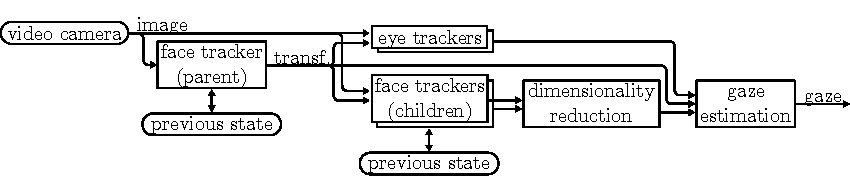
\includegraphics{img/impl-overview.pdf}
	\caption{Overall scheme of gaze tracking.}\label{i:impl-overview}
\end{figure}

The pipeline of computation is presented in Drawing \ref{i:impl-overview}.
Firstly, the face is locally tracked from the previous frame by the so-called parent tracker.
Only if this step fails, the program executes a global face localization procedure.
This first step results in a geometric image transformation.

Next, the precise position of both eyes is established within a reasonable region in the face.
This step requires the face to be localized properly in the image but since the eyes can move very quickly, no information from previous frames is taken into account.

Finally, the 6 degrees of freedom of the head and the 2 degrees of freedom of each eye are fed into a gaze estimator that outputs coordinates in screen reference frame.

\section{Face Tracking}
\label{s:impl-face}

\textit{Input:} reference image $\textrm{R}$ and current image $\textrm{I}$.\\
\textit{Output:} geometric transformation $T: \R^2 \to \R^2$ such that $\int_{\vec p} |\textrm{R}(\vec p) - \textrm{I}(\textrm{T}(\vec p))|^2$ is minimal.\footnote{
Because we do not actually intend to use integral calculus, the integral is only written in an informal way.
The full form would read: $\int_{\vec p \in \Omega} |\textrm{R}(\vec p) - \textrm{I}(\textrm{T}(\vec p))|^2 \mathrm{d}\vec p$, where $\Omega$ is the image domain.
}\\

The tracking is split into two parts: a \textit{parent tracker} that covers the whole face, and several \textit{child trackers} that capture more subtle degrees of freedom.
All of the trackers are deformable templates along the lines of \cite{bouguet01}.

The parent tracker provides a reference frame for all other features (e.g., eye trackers) and it supplies the most important parameters to gaze estimation.
In order to gain some robustness against changes in lighting, the parent tracker is color-normalized.

A surface within the face is tracked pixel per pixel, minimizing the energy function
$$\int_{\vec p} |\textrm{R}(\vec p) - \textrm{I}(\textrm{T}(\vec p))|^2,$$
where $T: \R^2 \to \R^2$ is a differentiable image transformation.
The reference image $R$ is a single frame that is used during the whole course of operation.
Although this approach does not tolerate long term changes (such as when the user takes on their glasses), it is robust against slow drift.

Depending on the motion model expressed by the transformation, we get different kinds of trackers:
\begin{itemize}
\item Similarity transformation. 4 DoF. Aligning in grid makes no sense at all.
\item Affinity over a triangle. 6 DoF. Possible to align in grid.
\item Affinity over a quadrangle. 6 DoF. Aligning in grid makes no sense.
\item Homography. 8 DoF. Possible to align in grid. Appropriate from a theoretical standpoint.
\end{itemize}
For performance reasons, a motion model must be chosen at compilation time, and it is shared by all the trackers.

We discretize the formula as a pixel-by-pixel sum and optimize it by gradient descent.
The derivatives of the transformation are computed analytically.
In case of the two motion models that are possible to align in grid (the triangle affinity and the homography), the derivatives are considered interesting enough and have been described in sections \ref{s:algo-daffine} and \ref{s:algo-dhomo}, respectively.
The remaining two use only simplistic formulas that have been omitted.

In order to allow large-scale movement, all of the trackers operate upon an \textit{image pyramid}.
\todo{define the pyramid}

Our program supports two methods how the child trackers are managed.
These represent two major groups of tracking techniques in general: the feature-based and the appearance-based method.

\subsection{Markers}

This method relies on small-scale features that are usually present in the face and on skin---such as the eyebrows, nostrils, beard and skin defects.
Several small trackers are arbitrarily placed within the face area, each of them large just enough so as to track a single feature of the face.
Technically, it is possible to track any distinctive texture, so an automated feature detection such as the Harris corner detector (provided by a third-party library) performs well enough.

Each of the markers is allowed to freely move around.
(In contrast to the classical Deformable Parts Model such as in \cite{uricar12}, we do not calculate any penalty from their relative configuration.)
They are tracked from their previous known position relatively to the parent tracker.
If the tracking score of a marker drops below a certain limit or a marker escapes the face area, it is reset to its original position and tracking continues from there.

\subsection{Grid}

This method follows the approach of Active Appearance Models \cite{cootes01}.
The parent tracker is subdivided into a planar mesh, and each cell is responsible of tracking the corresponding part of the image.

In order for the cells to form a contiguous mesh, certain parameters of neighboring cells are bound together and need to be optimized concurrently.
Our implementation of the corresponding tracker methods does this explicitly since their parameters are the planar coordinates of their corner vertices.
During optimization, the derivatives are summed up in each grid vertex (nevertheless the number of cells that share it) and all grid vertices are updated at once.

This process is commonly done with a triangular mesh (i.e., barycentric cells), where the derivatives wrt. vertex coordinates are quite easy to derive.
Our extension of this method to a quadrangular mesh (i.e., homographic cells) relies on the theory developed in Section \ref{s:algo-dhomo}.

\section{Eye Tracking}

\textit{Input:} iris radius $r \in \R$ and image $I$ centered at an expected eye location.\\
\textit{Output:} iris center $\vec c \in \R^2$.\\

\todo{further assumptions on the image necessary for good recognition}
\todo{list out the difficult factors and reference the table in Results}

Once the face itself has been tracked, the eyes can be easily located using their reference position.
The iris radius can also be extracted by multiplying the reference radius with a scale factor given by the face tracker.
Most of the face trackers induce non-uniform scaling, so it might seem appropriate that the eye shape will be an ellipse.
However, we assume that eyes are always directed towards the camera, so the limbus should retain a circular shape even if the face is stretched.

\todo{explain that we do not impose many constraints on the pupil occlusion, so the problem is actually very hard.}

There are a plenty of eye trackers available in our program.
From a broader perspective, we took four different approaches:
\begin{itemize}
\item Tracking the limbus. There should be a circle with a strong gradient directed outwards.
\item Tracking the iris. It should be radially symmetric with a strong gradient on the edges.
\item Segmentation. Skin, sclera, iris and pupil should each be uniform, but mutually different in color.
\item Machine learning. Instead of modeling, we can feed the image into a regression engine.
\end{itemize}

Acknowledging that the scale (e.g., the radius $r$) can be only a few pixels, we aim for a subpixel precision.
That is a meaningful pursuit thanks to the continuous image model defined in Section \ref{s.imagemodel}.

However, many of the algorithms to be presented are based on pixel by pixel evaluation of a scoring function.
In such cases, it is not very appropriate to evaluate at fractional coordinates.
Instead, we fit a quadratic polynomial to several score values around the maximal pixel, and output the maximum of this polynomial as the global maximum.

The following methods are available to the host application:

\subsection{Limbus gradient}
This method relies on the edge between the iris and the sclera.
Assuming that the iris is much darker than the sclera, their shared boundary (the limbus) should be sensed as a circle of high contrast.
Curve fitting to detected edge pixels can provide very precise results \cite{kassner14}.
Given the image resolution we work with, the usual approach based on a Canny filter and ellipse fitting is not viable.
Instead, we propose an iterative optimization scheme that will directly fit a circle to the image gradient.

We assume the eyelids be of uniform color, so they have zero value in the gradient domain and can be neglected.

\todo{formulate the energy function}
This function is minimized by gradient descent.
It is important to note that optimization of a function based on image gradient requires image derivatives of second order to be calculated.
\todo{if there is a citation for this:}
These are often considered unstable and avoided in the literature.
In our case, the function to be optimized appears to be smooth enough, and the algorithm converges well if initialized a few pixels from the correct solution.

This method is designed for refining an estimated eye position on the subpixel level, so it performs well when coupled with another eye tracking method.
If executed alone, it often fails to locate the global optimum.

\subsection{Hough Transformation}
We can use a voting scheme to find the limbus center, as described in Section \ref{s:algo-hough}.
\todo{used in \cite{leo14,zhang13}}

A free parameter is yet to define: the resolution of the voting grid.
Using each pixel as a voting bin is usually the best choice, but it may fail on blurry images of high resolution because the votes will be distributed quite randomly over a wide region around the true center.

\subsection{Dark iris correlation}

Assuming that the iris is a dark disc and the rest of the image is much brighter, we can use basic template matching techniques to locate it.
This technique is very popular \cite{zhu12,george16}
An appropriately fast and reliable one is the normalized correlation, using a slightly blurred black circle as the template.

\todo{formula for the kernel}

This method appears to work especially well when tested in regions where the majority of people are brown-eyed and with white skin.
It can also easily get confused by dark spots around the eyes, such as glass rims or strong makeup.
Finally, this method requires most of the iris to be visible, which need not be true because of the viewing angle and the user's personal habit.

\subsection{Personalized iris correlation}
The assumption of dark iris is wrong: the iris is often much brighter than the surrounding skin, especially in the case of blue-eyed people.
In fact, the iris image varies so greatly among individuals that it is often advocated as a means of identification or authentification \cite{bowyer16}.
We can, however, rely on the whole iris region (including the pupil) to be a constant, radially symmetric image, and locate it using a personalized template.
Acquiring this template requires the user to wide open their eyes, so that the whole limbus is visible.

For tracking a colored object, it is again reasonable to use the normalized correlation.

\subsection{Iris radial symmetry}

It may be considerably difficult to obtain a reliable iris image, and generally speaking it is a calibration step that we wish to avoid.
Instead, we can use the sole fact that the iris is a radially symmetric object on a white background.
An example of a filter based on radial symmetry can be found in \cite{leo14}.
Hereby we design a novel robust algorithm that exploit color information.

The iris colors are recalculated for each frame and each eye position, so only few free parameters remain.

This algorithm has built-in skin masking, so that whole segments of the iris are ignored where the limbus is not visible.

\todo{Add some intro -- let us define the following functions}
\begin{itemize}
\item
Angular limbus score $\textrm{limbus}(\alpha)$ is the gradient magnitude $|\nabla \textrm{I}(\vec p)|$ where $\arctan(\vec p) = \alpha$ and $|\vec p| = r$.

\item
Radial color $\textrm{mean}(t)$ is a mean value of the set $\{\textrm{I}(\vec p) \text{ for all } |\vec p| = t \}$.

\item
Angular iris score $\textrm{iris}(\alpha)$ is the weighted arithmetic mean of the set $\{\textrm{I}(\vec p)$ for all $\arctan(\vec p) = \alpha \}$.
The weight is $\textrm{w}(\vec p) = t \cdot (c - |\textrm{image}(\vec p) - \textrm{mean}(t)|)$, clamped to zero, with $t = |\vec p|$ and $c$ being a value appropriately chosen.

\end{itemize}
The total score is defined as $\int_\alpha \textrm{limbus}(\alpha) \cdot \textrm{iris}(\alpha)$.

Note that the formula for $\textrm{mean}(t)$ has not been specified yet.
Using the arithmetic mean may have a bad impact on the overall success rate.
It is appropriate here to use a more robust formula such as the median.

There are essentialy two ways how to generaze the median to color pixels.
Firstly, we can pick the median value as sorted by a scalar value (e.g., brightness).
This approach becomes unpredictable if many different colors have the same brightness, and specifically in the case of skin tones and iris color, this may be an issue.

The second option is to define the median of set $S$ as the value $\vec m \in S$ such that the sum of distances $\sum_{\vec x \in S} |\vec m - \vec x|$ is minimized.
This formula is consistent with the one-dimensional case and is valid in any metric space.
Unfortunately, efficient algorithms to compute this value are too sophisticated, so we loop over $S$ explicitly.

This function is computationally expensive and, depending on the method for mean color calculation, difficult to optimize locally.
Our program does not even contain the code to calculate the derivatives.
This tracker uses exhaustive search to find the global minimum within a crop-out image.

\subsection{Skin masking}

Skin, including the eyelids, can be detected quite easily by an analysis of its color.
This approach is perhaps too naive to be widely advocated in the literature, but it can be found in software libraries such as \cite{deepgaze}.

We allow each of the eye trackers presented so far to be coupled with a HSV (hue-saturation-value) detector tuned for skin tones.
Pixels whose HSV vector lies within a user-defined cube are excluded from eye fitting.

The mapping of RGB values to HSV is a piecewise linear function:
\todo{formula}

It is important to note the heuristic aspects of this approach.
\todo{HSV, sRGB, the cube -- lighting, skin color etc.}

Since there are usually many distractive features around the eyes, such as the eyelashes and makeup, the mask is pre-processed so as to have a smooth boundary and to cover nearby black splotches.

\todo{This is yet to be coded and tested.}

\subsection{Combined estimator}

Having implemented several algorithms for the same task, it is possible to adaptively combine their results.
An example of two different algorithms summing their results can be found in \cite{leo14}.
A more common approach is to run several trackers in sequence, such as in \cite{wang16,george16,zhu12}.
Our program supports can combine both of these options in a tree-like manner arbitrarily.

Choosing several trackers that are sensitive to different deteriorations of the image, we can trade off some computational time for much robustness and precision.
Each of the trackers chosen should obviously fail in different conditions so that a majority of them is correct on every image.
For an empiric comparison on reasonable selection of trackers for a combined estimator, see Section \ref{s:results-eyecovar}.

After letting each of the selected trackers cast a vote, it is possible to combine them robustly (as compared to the arithmetic average).
It is very much possible that one or more of the trackers fail.
We have very little prior information about the eye position, but we can exploit the distances among the votes.

In the case of three trackers running in parallel, we can heuristically throw out the vote that is significantly far away from the remaining two.
For a higher count of votes (assuming still that the number is reasonably small), this can be generalized as the subset with minimal expected variance.
In order to find it, we explicitly loop over all the subsets.
The average of this subset is the result of the combined estimator.

Note that in the case of two votes, their arithmetic mean is the only option.
In the three-vote case, either a mean of two or the mean of all three can be selected depending on their relative distances.

\begin{lemma}
Given a set $\{\vec x^i\}$ of samples from a normal distribution $X$, the expected value of the variance $\var X$ is
$$\E\var (\vec x) = \frac 1 {n - 1} \sum_i (\vec x^i - \hatvec x),$$
where $\hatvec x$ is the arithmetic mean.
\end{lemma}
\begin{proof}
\todo{cite or derive}
\end{proof}

Another option is to run several algorithms in sequence.
In this setting, the first algorithm provides a rough estimate that is subsequently refined by the remaining ones.
Since most of our eye trackers use exhaustive pixel-by-pixel search, there are only few meaningful configurations of this kind.

\section{Gaze estimation}
\label{s:impl-gaze}

\textit{Input:} vectors $\vec e \in \R^n$ and $\vec f \in \R^m$ and \textit{gaze parameters} as defined below.\\
\textit{Output:} vector $\vec p \in \R^2$.\\

\begin{definition} \label{d:gaze-parameters}
The \textit{gaze parameters} consist of an orthonormal basis $\mat P \in \R^{2\times n}$ and a homography $\mat H \in \R^{3 \times (m+3)}$.
\end{definition}

Given the vector $\vec f$ obtained from face tracking and vector $\vec e$ obtained from eye tracking, and using the scene model described in Section \ref{s:gaze-model}, we wish to estimate the on-screen position $\vec p$ (in pixel units).
Commonly used approximation methods for this purpose vary greatly from simple approximations \cite{zhu12} more flexible ones \cite{kassner14,yucel09} and thorough geometric models \cite{villanueva08,wang16}.

Computer screen is a plane in space, with pixels aligned in a regular square grid.
If the face and the eyes were also planar objects, then the gaze in screen coordinates would be related to the face and eyes position by a projectivity.
This is obviously not the case, and the face transformation has many more degrees of freedom than a planar rigid body would.
 
In order to properly model the mapping from our face and eye parameter space to two-dimensional gaze, we would have to actually approximate the three-dimensional model of the face.
Many programs have been published (e.g., \cite{fanelli11}) that follow this path.
In general, it requires some prior information about the shape of the face, and much tuning to calibrate a 3d model precisely enough.
To avoid these issues, we decided for a simpler approach.

We decided to actually assume the gaze is given by a projective transformation of the face and eye parameters.
This approach is limited and even in theory, it does never perfectly fit the data.
On the other hand, homographies have a solid mathematical background, and they can be estimated quickly and robustly from data.
All invertible homographies form a group that contains the group of invertible affine transformations, and they can also implicitly model inverse proportionalities among their parameters.


\todo{combine with the following section in a meaningful manner}

\section{Calibration}

\textit{Input:} interactive session with the user.\\
\textit{Output:} gaze parameters (see Definition \ref{d:gaze-parameters}).\\

The purpose of calibration is to learn all necessary parameters about the user's face and the geometry of the screen relatively to the camera.
Depending on the tracking quality, the time spent to measure all necessary information may vary.

During the calibration, roughly speaking, the user is asked to watch specific points on screen and their face and eyes are tracked.
For each screen position measured this way, the face tracker provides many parameters.
Some of these have an implicit meaning, others can be processed to extract useful information and yet others are just noise.
We fit a homography mapping some of the face parameters and the eye parameters to each known gaze position.

In the beginning of the calibration session, a single frame is acquired from the camera.
Depending on the application, either the program locates the user's face and eyes, or asks the user to do so manually.
For the automatic face and eye localization, a boosted random forest classifier is used within a sliding window.

The calibration session proceeds by presenting the user with a dot moving around the screen.
The user is asked to watch the dot carefully until it disappears.
In order to make the movement more predictable, the dot moves along a smooth curve with piecewise constant curvature, and a patch of this curve is being drawn ahead of time.
The calculated parameters from face tracking are recorded along with the current on-screen position of the dot.

It is meaningful to extract four basic parameters about a face tracker: its position within the image, its on-screen rotation and scale.
The head (as a rigid body) has two more parameters to be covered, but there is a virtually unlimited number of extra parameters that can be obtained from detailed tracking of the face.
Face pose is unknown in each frame, and possibly constant, so there is a high danger of overfitting.
We cut down the dimensionality by Principal Component Analysis: out of the extra parameters, only the two largest principal components are preserved.

It is possible that the user's gaze twitches for a moment, or that the gaze tracking fails in several frames.
In order to ignore these faulty measurements, we employ a Ransac fitting repetitively.
As soon as a fit collects a large enough support of measurements, the calibration procedure stops and outputs the homography it acquired.


\chapter{Results}

Having designed and implemented the gaze tracker, we shall now evaluate its performance.
There are three aspects to consider when talking of performance: robustness, precision and speed.

\section{Face tracking}
Let us introduce the transformations available in face tracking by an example of two still images:
\todo{intuitively compare the face tracking methods on a real image}

\todo{explain that a more thorough comparison is not possible because the planar transformation between two faces is not clearly defined.}

\section{Eye tracking}

For a start, we compared the overall performance on all data available.

There are two combined trackers in addition to all the simple ones.

The one called \textit{h;l} is a Hough tracker and a Limbus gradient tracker running in series, in this order.

In the tracker called \textit{chr;l}, we replaced the simple Hough tracker with a parallel combination of Correlation, Hough, and Radial trackers.
Again, the result is refined by the Limbus gradient tracker afterwards.

\begin{table}[h]
\centering
\begin{tabular}{l@{\hspace{1.5cm}}D{.}{.}{3.2}}
\toprule
\textbf{Algorithm} & \mc{\textbf{Mean [px]} \todo{Q1, Q2, Q3}} \\
\midrule
h;l & 7.30 \\
hough & 8.26 \\
chr;l & 11.97 \\
radial & 12.11 \\
correlation & 16.48 \\
bitmap & 28.55 \\
limbus & 35.23 \\
\bottomrule
\end{tabular}
\caption{Algorithm mean error}\label{t:algo-mean}
\end{table}

Looking at the quartiles Q1 and Q2, it seems that there are many nice cases where the algorithms perform much better.
Indeed, the results of \textit{h;l} combined tracker look like this:\\
\todo{graph.}

We evaluated the algorithms separately on each of our data sets:\\
\todo{table.}

We also selected a subset of the test images with high contrast and limited occlusion:\\
\todo{table.}

Apparently, the simple tracker based on Circle Hough Transformation provides the best result.
Its performance can be improved at subpixel scale by adding an additional step of the Limbus gradient maximization.

It is quite disappointing that a voting scheme based on three of our trackers appears to perform worse than the best of them.

We should note that our Radial tracker is considerably slower than all the remaining ones.
On overly large-resolution images, its execution time can actually harm the overall framerate of gaze recognition.
\todo{edit this when the results are done.}

\subsection{Failure factors}
\label{s:results-eyecovar}

Apparently, the results of eye tracking depend heavily on the qualitative aspects of each image.
For this reason, we annotated each of our testing samples in the following regards:
\begin{itemize}
\item Iris brightness
\item \todo{more}
\end{itemize}
The quantities are expressed in a subjective scale from $1$ (effect not visible) to $3$ (severe impact) or $4$ (image is almost unrecognizable).
Apart from this, each eye sample has already been labeled with the iris radius.

As expected, there is a strong correlation between many of these quantities:
\begin{table}[h]
\centering
\begin{tabular}{l@{\hspace{1.5cm}}D{.}{.}{3.2}D{.}{.}{3.2}D{.}{.}{3.2}D{.}{.}{3.2}}
\toprule
\textbf{Algorithm} & \mc{\textbf{Size}} & \mc{\textbf{Iris}} & \mc{\textbf{Contrast}} & \mc{\textbf{Glare}}\\
\midrule
h;l & 21.44 & 0.17 & -0.14 & -0.49\\
hough & 16.68 & -0.11 & -0.09 & -0.49\\
chr;l & 33.03 & 1.80 & 0.19 & 0.73\\
radial & 37.92 & 0.61 & 0.02 & 0.76\\
correlation & 34.09 & 3.30 & -0.06 & 1.29\\
bitmap & 72.23 & 0.74 & 0.54 & 1.43\\
limbus & 46.57 & 0.54 & 0.37 & 0.41\\
\bottomrule
\end{tabular}
\caption{Covariance of mean error wrt. image properties}\label{t:algo-covar}
\end{table}

For completeness, we repeated this test with each of our 
\todo{repeated for each of the three data sets, referenced to the attachment for their description}

\section{Gaze Estimation}
\todo{the overall success rate of the algorithm on the videos from Tobii}\\
\todo{compare two trackers $\times$ two face trackers}

The program does not perform all that well when compared to the state of the art, but it is certainly much more than a proof of concept.

The results on flawless video streams are already usable, and challenging situations could perhaps be solved with more coding manpower.
\todo{\dots}

\chapter*{Conclusion}
\addcontentsline{toc}{chapter}{Conclusion}


%%% Bibliography
%%% Bibliography (literature used as a source)
%%%
%%% We employ bibTeX to construct the bibliography. It processes
%%% citations in the text (e.g., the \cite{...} macro) and looks up
%%% relevant entries in the bibliography.bib file.
%%%
%%% The \bibliographystyle command selects, which style will be used
%%% for references from the text. The argument in curly brackets is
%%% the name of the corresponding style file (*.bst). Both styles
%%% mentioned in this template are included in LaTeX distributions.

\bibliographystyle{plainnat}    %% Author (year)
% \bibliographystyle{unsrt}     %% [number]

\renewcommand{\bibname}{Bibliography}

%%% Generate the bibliography. Beware that if you cited no works,
%%% the empty list will be omitted completely.

\bibliography{bibliography}

%%% If case you prefer to write the bibliography manually (without bibTeX),
%%% you can use the following. Please follow the ISO 690 standard and
%%% citation conventions of your field of research.

% \begin{thebibliography}{99}
%
% \bibitem{lamport94}
%   {\sc Lamport,} Leslie.
%   \emph{\LaTeX: A Document Preparation System}.
%   2nd edition.
%   Massachusetts: Addison Wesley, 1994.
%   ISBN 0-201-52983-1.
%
% \end{thebibliography}


%%% Abbreviations used in the thesis, if any, including their explanation
%%% In mathematical theses, it could be better to move the list of abbreviations to the beginning of the thesis.
%\chapwithtoc{List of Abbreviations}

%%% Attachments to the master thesis, if any. Each attachment must be
%%% referred to at least once from the text of the thesis. Attachments
%%% are numbered.
%%%
%%% The printed version should preferably contain attachments, which can be
%%% read (additional tables and charts, supplementary text, examples of
%%% program output, etc.). The electronic version is more suited for attachments
%%% which will likely be used in an electronic form rather than read (program
%%% source code, data files, interactive charts, etc.). Electronic attachments
%%% should be uploaded to SIS and optionally also included in the thesis on a~CD/DVD.
\chapwithtoc{Attachments}

\setcounter{section}{0}
\stepcounter{chapter}
\renewcommand{\thesection}{\Alph{section}}

\section{Directory structure of the attached data}
\label{s:dirstructure}
\begin{itemize}
\item The directory {\tt bin/} contains \dots

\item {\tt doc/install.html} and {\tt doc/usage.html} is the user documentation of the program.
The file {\tt doc/code.html} contains developer documentation and overall notes about the structure of the code.

\item {\tt extern/} contains the less common external libraries that are needed to compile and run the program.

\item {\tt src/} contains the whole source code of the program.
Apart from it, a Python script {\tt src/io\_export\_tracks.py} is provided that serves for exporting the camera calibration conveniently from Blender as input to our program.
Further files for testing of the source code are provided in {\tt src/test/}.

\item The directory {\tt data/} contains data for testing of the program.

\item Finally, the file {\tt thesis.pdf} is the electronic version of this document.

\end{itemize}

\section{Library interface}

The software can be readily used as a gaze tracking library.
There are a few decisions that the host application must make in order to initialize the tracking algorithms.
\todo{\dots}

The file {\tt src/example\_main.cpp} is a simple gaze tracking application and an example of the application interface.
There are more similar files prefixed with {\tt example\_} that showcase smaller bits of the code, and often use methods that should be hidden from the host application.


\openright
\end{document}
